%%%%%%%%%%%%%%%%%%%%%%%%%%%%%%%%%%%%%%%%%%%%%%%%%%%%%%%%%%%%%%%%%%%%%%%%
% Plantilla TFG/TFM
% Escuela Politécnica Superior de la Universidad de Alicante
% Realizado por: Jose Manuel Requena Plens
% Contacto: info@jmrplens.com / Telegram:@jmrplens
%%%%%%%%%%%%%%%%%%%%%%%%%%%%%%%%%%%%%%%%%%%%%%%%%%%%%%%%%%%%%%%%%%%%%%%%

\chapter{Análisis, Especificación y Diseño}
\label{analisis}

\section{Requisitos del sistema}
En esta sección se detallan los requisitos del sistema, divididos en requisitos funcionales, no funcionales y de configuración. Los requisitos se han estructurado en formato tabular para facilitar su comprensión y seguimiento durante el desarrollo del proyecto.

\subsection{Requisitos funcionales}
Los requisitos funcionales describen el comportamiento que debe tener el sistema, las funcionalidades que debe ofrecer y las operaciones que debe realizar.

\begin{table}[H]
\centering
\begin{tabular}{|p{1cm}|p{4cm}|p{9cm}|}
\hline
\textbf{ID} & \textbf{Nombre} & \textbf{Descripción} \\
\hline
RF-01 & Detección de ficheros & El sistema debe detectar nuevos ficheros en el directorio observado. \\
\hline
RF-02 & Diferenciación de tipos & El sistema debe diferenciar el tipo de archivo a analizar (texto, imagen, vídeo, audio, otros). \\
\hline
RF-03 & Ejecución de modelos & El sistema debe ejecutar el modelo correspondiente que extraerá la información del fichero a la base de datos. \\
\hline
RF-04 & Almacenamiento & El sistema debe almacenar todos los datos posibles sobre el fichero analizado en una base de datos. \\
\hline
RF-05 & Interfaz web & El sistema debe tener una interfaz web super-simple donde el usuario podrá escribir su consulta en lenguaje natural y darle a un botón para realizar la búsqueda. \\
\hline
RF-06 & Resultados de búsqueda & El sistema responderá con un conjunto de resultados potencialmente interesantes a partir de la consulta de búsqueda, ordenados de más a menos "interesante". \\
\hline
RF-07 & Entrada por línea de comandos & El sistema debe tener una entrada por línea de comandos (ej: \texttt{LLMSearch --query "mapa del mundo en el que hay marcados los mejores parques naturales"}). \\
\hline
RF-08 & Presentación de resultados & El resultado será la ruta del fichero junto a una pequeña descripción del mismo (enlaces clicables al fichero y a la carpeta que lo contiene). \\
\hline
RF-09 & Inspección de archivos comprimidos & Los ficheros comprimidos deberían poder inspeccionarse por dentro. \\
\hline
RF-10 & Tipos de ficheros a procesar & El sistema debe procesar los siguientes tipos de ficheros: \\
& & - Documentos de texto \\
& & - Imágenes \\
& & - Vídeos \\
& & - Ficheros de sonido \\
& & - Otros (bases de datos, ejecutables, etc.) \\
\hline
\end{tabular}
\caption{Requisitos funcionales del sistema}
\label{tab:req_funcionales}
\end{table}

\subsection{Requisitos no funcionales}
Los requisitos no funcionales especifican criterios que pueden usarse para juzgar la operación de un sistema en lugar de sus comportamientos específicos.

\begin{table}[H]
\centering
\begin{tabular}{|p{1cm}|p{4cm}|p{9cm}|}
\hline
\textbf{ID} & \textbf{Nombre} & \textbf{Descripción} \\
\hline
RNF-01 & Configuración web & La web debe tener una pequeña parte de configuración discreta pero accesible en todo momento. \\
\hline
RNF-02 & Arquitectura modular & La arquitectura se debe dividir en un "buscador" y un "explorador" y deben ser completamente separadas para poder ser reutilizadas. \\
\hline
RNF-03 & Ejecución sin GPU & El sistema debe poder ejecutarse en un ordenador sin GPU (opcional). \\
\hline
RNF-04 & Parámetro de consulta & La entrada por línea de comandos aceptará un parámetro \texttt{--query} junto al término de búsqueda. \\
\hline
RNF-05 & Resultados en CLI & La entrada por línea de comandos devolverá los resultados de la misma manera que el buscador web con la diferencia de que solo devolverá información adicional si se le añade el parámetro \texttt{--verbose}. \\
\hline
RNF-06 & Estado del sistema & La entrada por línea de comandos tendrá un parámetro \texttt{--status} que devolverá el estado del sistema: número de archivos procesados sobre el número total de archivos en observación, cantidad de ficheros de cada tipo, errores encontrados... \\
\hline
RNF-07 & Configuración por CLI & Se añadirán los parámetros necesarios para poder configurar el sistema desde línea de comandos. \\
\hline
\end{tabular}
\caption{Requisitos no funcionales del sistema}
\label{tab:req_no_funcionales}
\end{table}

\subsection{Requisitos de configuración}
Los requisitos de configuración especifican las opciones que el usuario debe poder ajustar en el sistema.

\begin{table}[H]
\centering
\begin{tabular}{|p{1cm}|p{4cm}|p{9cm}|}
\hline
\textbf{ID} & \textbf{Nombre} & \textbf{Descripción} \\
\hline
RC-01 & Directorio de observación & Directorio donde se están observando nuevos ficheros. \\
\hline
RC-02 & Regulación de carga & Regular la carga (limitar la CPU al X\%). \\
\hline
RC-03 & Tipo de modelo LLM & Tipo de modelo LLM a utilizar (Local \textit{(LLM Studio)} ó en la nube). \\
\hline
RC-04 & Búsqueda por imagen & Posibilidad de poner una foto de una persona y que la busque en los ficheros. \\
\hline
\end{tabular}
\caption{Requisitos de configuración del sistema}
\label{tab:req_configuracion}
\end{table}

\section{Arquitectura del Sistema}
\label{sec:arquitectura_sistema}

La arquitectura de LLMSearch se ha concebido como un sistema modular y distribuido, con el objetivo de facilitar la escalabilidad, el mantenimiento y la posible reutilización de componentes. Un esquema visual inicial de esta arquitectura se presenta en la Figura \ref{fig:arquitectura_general}.

\begin{figure}[H]
  \centering
  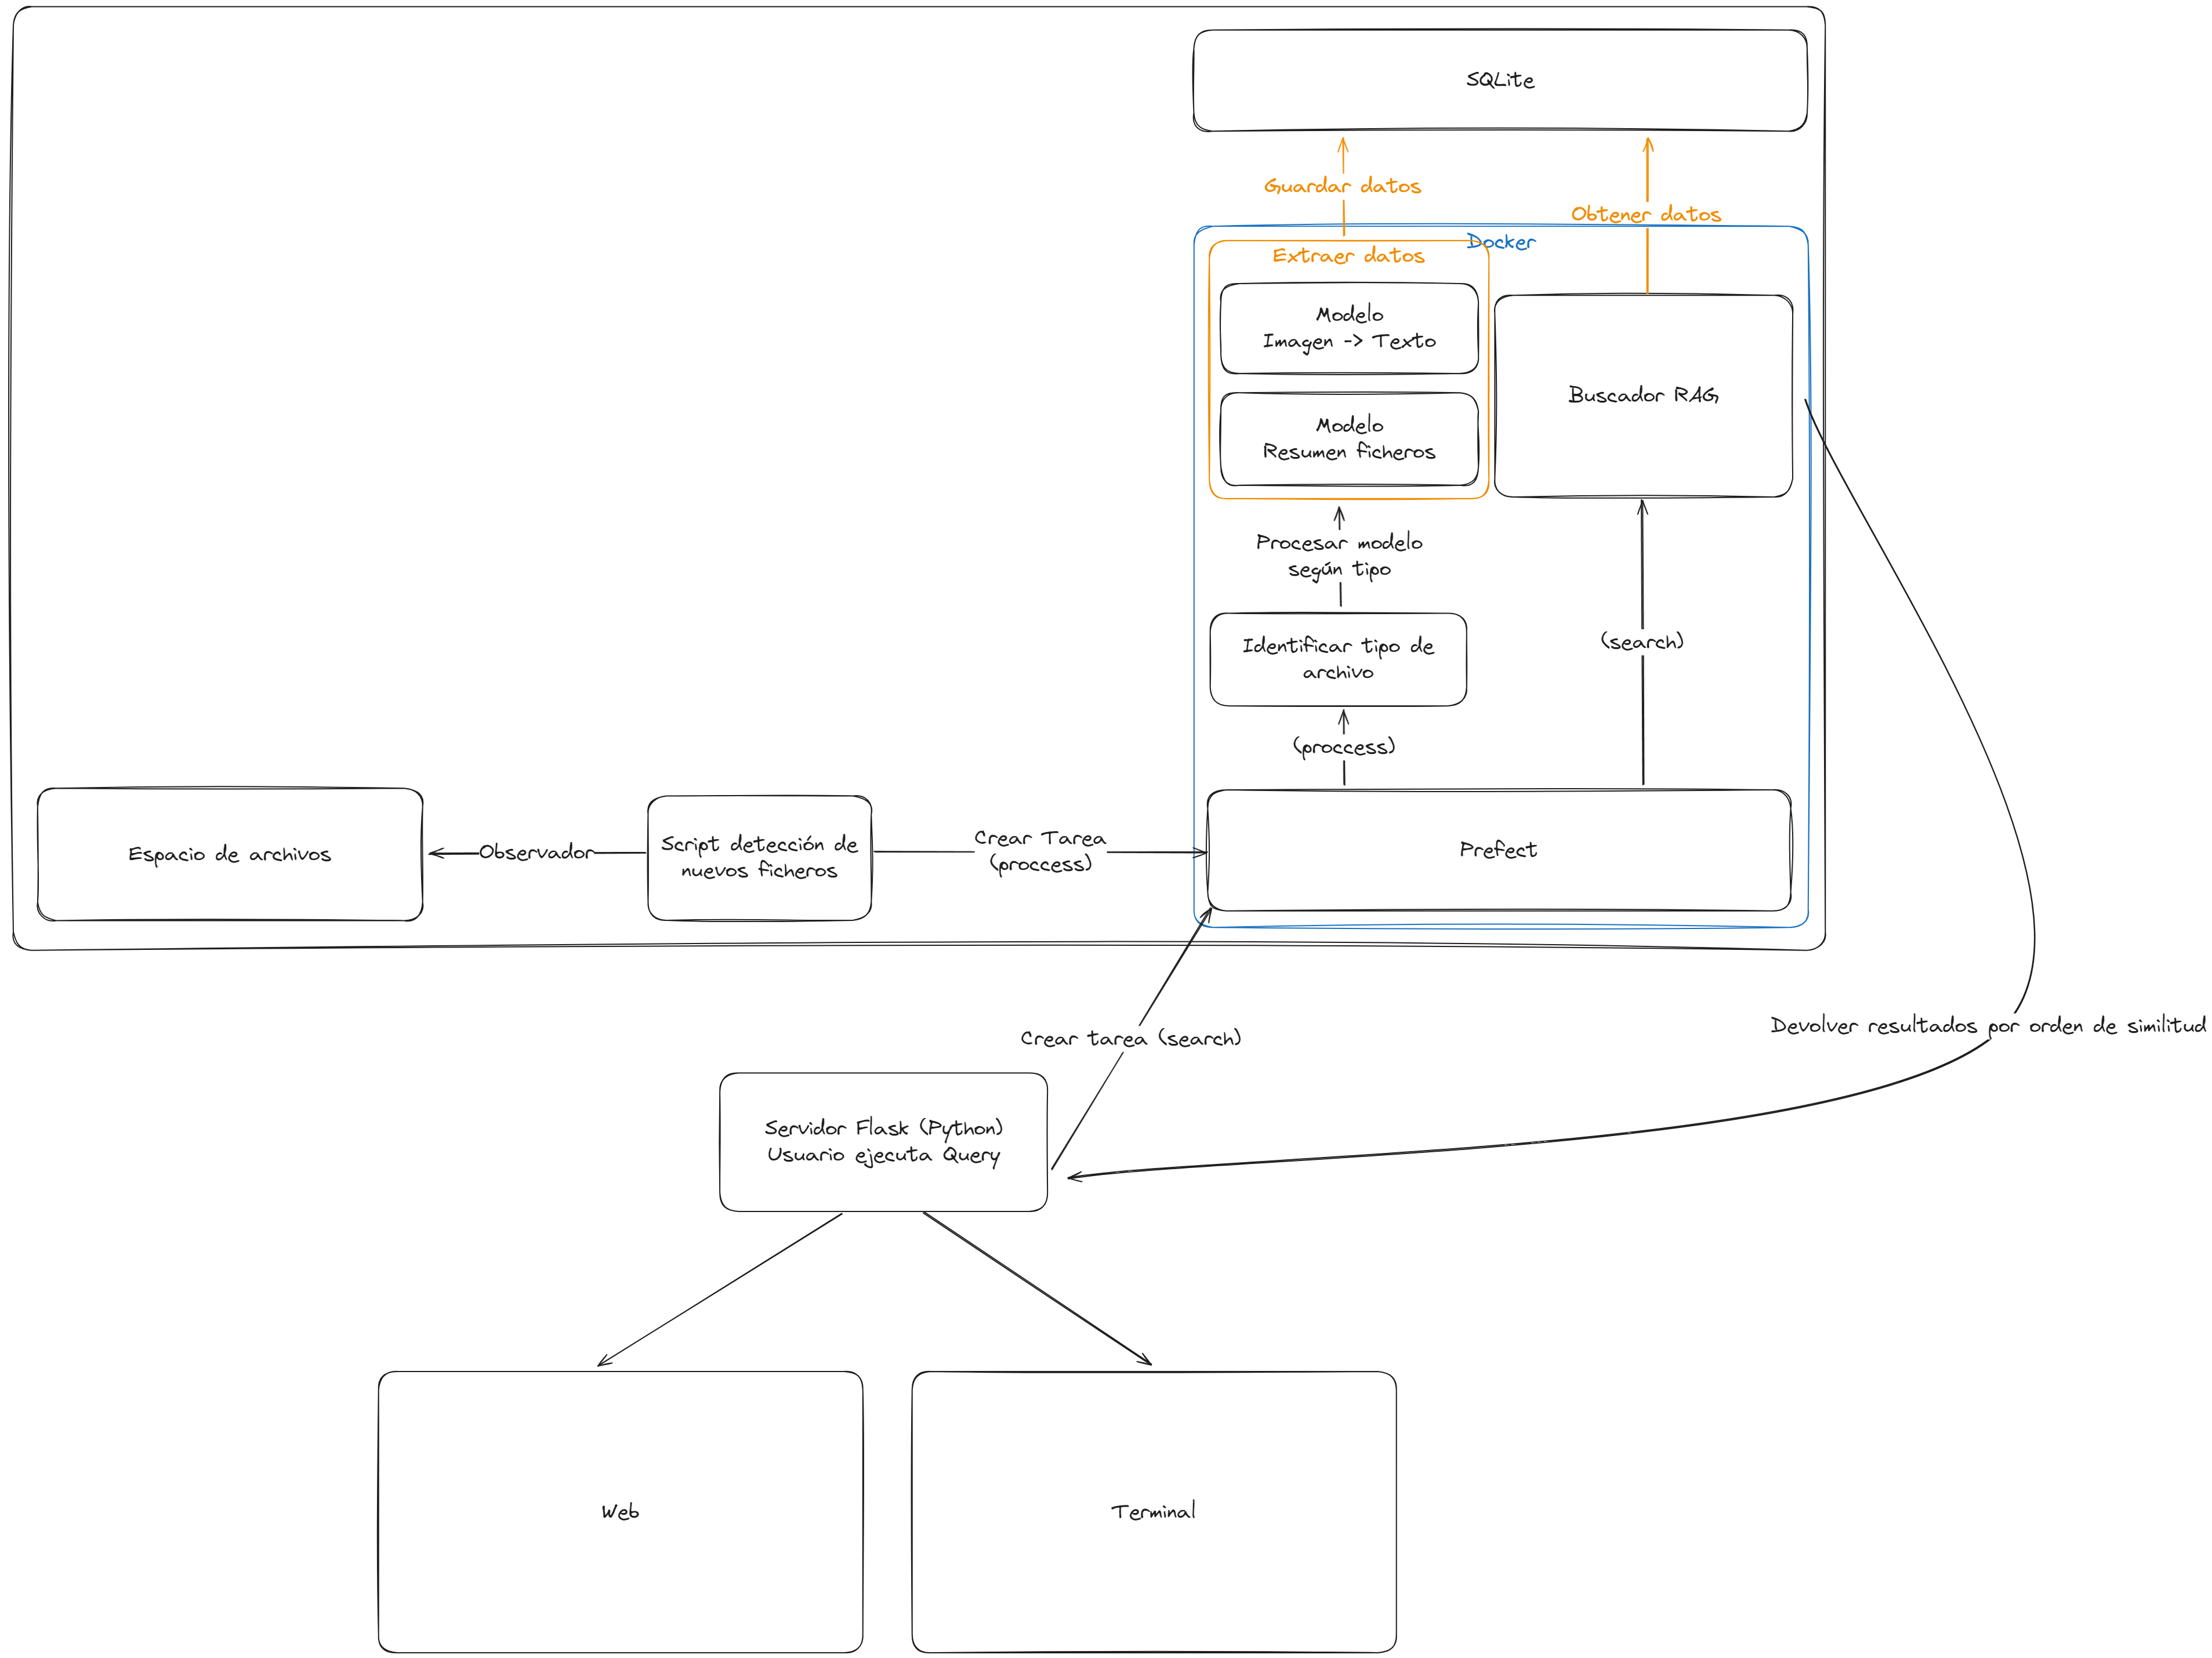
\includegraphics[width=\textwidth]{archivos/arquitectura.png}
  \caption[Arquitectura de LLMSearch]{Diagrama de la arquitectura general de LLMSearch.}
  \label{fig:arquitectura_general}
\end{figure}

Es importante señalar que el diagrama de la Figura \ref{fig:arquitectura_general} representa una instantánea conceptual de las primeras etapas del diseño del proyecto. Si bien captura la esencia de la modularidad y los flujos principales, ciertos componentes y sus interacciones han sido refinados o modificados durante el proceso de desarrollo para optimizar el rendimiento, la simplicidad o la adecuación a las herramientas finalmente seleccionadas. Por ejemplo, la especificación y el tipo de la base de datos han evolucionado desde la concepción inicial. Los siguientes apartados describen en detalle cada componente en su estado final de implementación, destacando las decisiones de diseño clave y cualquier desviación significativa respecto al esquema preliminar.

\subsection{Componentes Principales de la Arquitectura}

\begin{itemize}
    \item \textbf{Script Observador}:
    Este componente es el encargado de monitorizar de forma continua el directorio o directorios especificados por el usuario (según RC-01) en busca de nuevos ficheros o modificaciones en los existentes (RF-01). Cuando detecta un cambio relevante, el observador notifica al servidor para iniciar el proceso de análisis del fichero.

    \item \textbf{Servidor Central (Backend API)}:
    El núcleo del sistema reside en una aplicación servidor que actúa como punto central de comunicación y control. Sus responsabilidades principales son:
    \begin{enumerate}
        \item Inicializar y gestionar el ciclo de vida del \texttt{Script Observador}.
        \item Recibir notificaciones del observador sobre nuevos ficheros o ficheros modificados.
        \item Exponer una \gls{api} RESTful para atender las peticiones provenientes tanto de la interfaz web (RF-05) como de la interfaz de línea de comandos (\gls{cli}) (RF-07). Estas peticiones incluyen las consultas de búsqueda de los usuarios y, potencialmente, comandos de gestión y configuración del sistema (RNF-07).
        \item Interactuar con el Orquestador de Tareas para delegar el procesamiento de ficheros y la ejecución de búsquedas.
    \end{enumerate}

    \item \textbf{Orquestador de Tareas}:
    Dada la naturaleza asíncrona y potencialmente intensiva en recursos del procesamiento de ficheros y las consultas a \glspl{llm}, se ha decidido incorporar un sistema de orquestación de tareas. Este sistema se encarga de la gestión de flujos de trabajo, permitiendo encolar tareas, ejecutarlas (posiblemente en procesos separados o workers), monitorizar su estado y gestionar reintentos o fallos. El servidor central enviará solicitudes de creación de tareas a este orquestador. Las tareas principales gestionadas por el orquestador serán:
    \begin{enumerate}
        \item \textbf{Tarea de Procesamiento}:
            Al recibir la ruta de un nuevo fichero, esta tarea coordinará varias subtareas:
            \begin{itemize}
                \item Invocará al \texttt{Identificador del Tipo de Fichero} para determinar la naturaleza del archivo (RF-02).
                \item En función del tipo, seleccionará y ejecutará el \texttt{Modelo de Extracción de Datos} correspondiente (RF-03).
                \item Paralelamente, se extraerán metadatos generales del fichero (nombre, tamaño, fechas, etc.).
                \item Finalmente, todos los datos extraídos (contenido semántico, metadatos) se persistirán en la \texttt{Base de Datos} (RF-04).
            \end{itemize}
        \item \textbf{Tarea de Búsqueda}:
            Cuando el usuario realiza una consulta, esta tarea:
            \begin{itemize}
                \item Recibirá la consulta en lenguaje natural del usuario como parámetro.
                \item Realizará una primera fase de recuperación de información relevante de la \texttt{Base de Datos}.
                \item Construirá un prompt optimizado, incorporando la información recuperada y la consulta original, para ser procesado por el \texttt{Buscador RAG} (utilizando un \gls{llm}).
                \item Devolverá un conjunto de resultados ordenados por relevancia o similitud con la consulta (RF-06).
            \end{itemize}
    \end{enumerate}

    \item \textbf{Identificador del Tipo de Fichero}:
    Para asegurar una correcta clasificación de los ficheros (RF-02) y evitar depender únicamente de la extensión (que puede ser engañosa o incorrecta), este módulo analizará las cabeceras o "números mágicos" de los ficheros para determinar su formato real. Se emplearán mecanismos especializados para una identificación robusta de una amplia variedad de tipos de archivo.

    \item \textbf{Modelos de Extracción de Datos}:
    Este es un conjunto de módulos especializados, cada uno diseñado para procesar un tipo específico de fichero (texto, imagen, vídeo, audio, etc., según RF-10). La arquitectura de estos modelos será eminentemente modular, permitiendo la fácil incorporación de nuevos extractores para formatos de archivo futuros o la actualización de los existentes. Cada modelo será responsable de invocar las herramientas de \gls{ia} o librerías pertinentes (ej. \gls{ocr} para imágenes, \gls{asr} para audio, análisis semántico para texto) para extraer la información significativa y estructurarla.

    \item \textbf{Base de Datos}:
    Para el almacenamiento persistente de la información extraída de los ficheros y los metadatos asociados (RF-04), se utilizará un sistema de base de datos. La elección de este sistema  basado en criterios de simplicidad, facilidad de configuración local (preferiblemente embebida, sin requerir un servidor de base de datos separado) y buena integración con el lenguaje de desarrollo principal. Se desarrollará una capa de acceso a datos para interactuar con la base de datos de manera estructurada y segura.

    \item \textbf{Buscador \gls{rag}}:
    El componente central para la búsqueda semántica (RF-06) se basará en la técnica de \gls{rag}. Este enfoque combina la recuperación eficiente de información de la \texttt{Base de Datos} con las capacidades de comprensión y generación de lenguaje natural de un \gls{llm}. Durante el análisis, se han considerado varias estrategias para implementar el \gls{rag}:
    \begin{itemize}
        \item \textit{Generación de Consultas SQL}: El \gls{llm} podría generar consultas \gls{sql} para interrogar directamente la base de datos. Si bien es una opción, presenta el riesgo de generar consultas subóptimas o incorrectas, y podría limitar la expresividad semántica si el \gls{llm} no comprende bien el esquema.
        \item \textit{Incorporación de Texto Completo al Prompt}: Convertir fragmentos relevantes de la base de datos a texto e incluirlos directamente en el prompt del \gls{llm}. El principal desafío aquí es la limitación de la ventana de contexto de muchos \glspl{llm}. Aunque modelos recientes (como algunos modelos chinos con ventanas de contexto muy amplias) podrían mitigar esto, requiere una filtración previa muy efectiva de la información de la base de datos para no exceder los límites o incurrir en altos costos computacionales.
        \item \textit{Uso de Embeddings para Contexto}: Transformar los datos recuperados y la consulta del usuario en embeddings (representaciones vectoriales) y utilizar estos embeddings para enriquecer el contexto del \gls{llm}. Esta suele ser la aproximación más eficiente y robusta, aunque puede implicar una mayor complejidad en la implementación de la infraestructura de embeddings y la gestión de la similitud vectorial.
    \end{itemize}
    La elección final de la estrategia \gls{rag} o una combinación de ellas dependerá de la experimentación y la evaluación del rendimiento y la complejidad.

\end{itemize}

\subsection{Consideraciones sobre Contenerización}
\label{subsec:docker_considerations}

Durante la fase de análisis, se evaluó la posibilidad de utilizar tecnologías de \textbf{contenerización} para los diferentes servicios del sistema. La contenerización ofrece ventajas significativas en términos de reproducibilidad del entorno, aislamiento de dependencias y simplificación del despliegue. Sin embargo, para la etapa actual del proyecto, y dado que el objetivo principal es desarrollar y validar la funcionalidad central en un entorno local, se ha optado por no implementar una solución de contenerización inicialmente. La gestión de dependencias a través de entornos virtuales específicos del lenguaje de programación y la configuración directa de los servicios en el sistema operativo local se considera suficiente y más ágil para el desarrollo iterativo. No obstante, la arquitectura modular propuesta facilitaría una futura migración a una infraestructura basada en contenerización si el proyecto escalara o se requiriera un despliegue en entornos más complejos.

\section{Casos de uso}
\label{sec:casos_de_uso}

Los casos de uso describen las interacciones típicas entre los actores (en este caso, principalmente el Usuario) y el sistema LLMSearch, mostrando cómo se utilizarán las funcionalidades principales para alcanzar objetivos específicos. Estos diagramas ayudan a visualizar el alcance funcional del sistema desde la perspectiva del usuario.

A continuación, se presentan dos diagramas de casos de uso: el primero ofrece una visión general de las interacciones principales del usuario, y el segundo detalla tipos específicos de búsqueda y opciones de configuración.

\begin{figure}[H]
  \centering
  \begin{tikzpicture}[scale=0.8, transform shape]
    \begin{UseCaseDiagram}
      % Actor
      \actor[x=-5, y=0]{Usuario}

      % Casos de Uso Principales
      \usecase[x=2, y=2.5]{Buscar Información en Ficheros}{CU1}
      \usecase[x=2, y=0]{Configurar Parámetros del Sistema}{CU2}
      \usecase[x=2, y=-2.5]{Consultar Estado del Sistema}{CU3}

      % Conexiones
      \connect{Usuario}{CU1}
      \connect{Usuario}{CU2}
      \connect{Usuario}{CU3}
      
      % Notas (opcional, para enlazar con Requisitos si se desea)
      % \node[note, right of=CU1, node distance=3.5cm] (N1) {Cubre RF-05, RF-06, RF-07, RC-04};
      % \node[note, right of=CU2, node distance=3.5cm] (N2) {Cubre RNF-01, RNF-07, RC-01, RC-02, RC-03};
      % \node[note, right of=CU3, node distance=3.5cm] (N3) {Cubre RNF-06};
    \end{UseCaseDiagram}
  \end{tikzpicture}
  \caption{Diagrama de Casos de Uso: Interacciones Principales del Usuario con LLMSearch.}
  \label{fig:casos_uso_general}
\end{figure}

El diagrama de la Figura \ref{fig:casos_uso_general} muestra las tres categorías principales de interacción que un usuario puede tener con el sistema: realizar búsquedas de información dentro de los ficheros procesados, configurar diversos aspectos del funcionamiento del sistema y consultar el estado actual del procesamiento de archivos.

El siguiente diagrama (Figura \ref{fig:casos_uso_detallados}) profundiza en las acciones específicas que el usuario puede realizar, especialmente en relación con los diferentes métodos de búsqueda y las opciones de configuración detalladas.

\begin{figure}[H]
  \centering
  \begin{tikzpicture}[scale=0.75, transform shape] % Ajustar escala si es necesario
    \begin{UseCaseDiagram}
      % Actor
      \actor[x=-8, y=0]{Usuario}

      % Casos de Uso de Búsqueda
      \usecase[x=-2, y=5]{Realizar Consulta Textual (Web)}{CU_SearchWeb}
      \usecase[x=-2, y=2.5]{Realizar Consulta Textual (CLI)}{CU_SearchCLI}
      \usecase[x=-2, y=0]{Buscar por Similitud de Imagen}{CU_SearchImage}
      
      % Caso de Uso Incluido/Extendido para Búsqueda
      \usecase[x=4, y=3.75, width=4cm]{Presentar Resultados de Búsqueda}{CU_PresentResults}
      \usecase[x=4, y=1, width=4cm, stereotype=extend]{Mostrar Información Detallada (CLI)}{CU_VerboseCLI}

      % Casos de Uso de Configuración
      \usecase[x=-2, y=-3]{Ajustar Directorio de Observación}{CU_ConfigDir}
      \usecase[x=3.5, y=-3, width=3.5cm]{Ajustar Límite de Uso de CPU}{CU_ConfigCPU} % Ajustado para evitar solapamiento
      \usecase[x=-2, y=-5.5, width=3.5cm]{Seleccionar Implementación de LLM}{CU_ConfigLLM}
      
      % Caso de Uso de Monitoreo
      \usecase[x=3.5, y=-5.5, width=3.5cm]{Verificar Estado del Sistema (CLI)}{CU_StatusCLI}  % Ajustado

      % Conexiones Actor -> Casos de Uso Principales
      \connect{Usuario}{CU_SearchWeb}
      \connect{Usuario}{CU_SearchCLI}
      \connect{Usuario}{CU_SearchImage}
      \connect{Usuario}{CU_ConfigDir}
      \connect{Usuario}{CU_ConfigCPU}
      \connect{Usuario}{CU_ConfigLLM}
      \connect{Usuario}{CU_StatusCLI}

      % Relaciones entre Casos de Uso
      \draw[umlinclude] (CU_SearchWeb) -- (CU_PresentResults) node[midway, above, sloped, scale=0.8] {\footnotesize <<include>>};
      \draw[umlinclude] (CU_SearchCLI) -- (CU_PresentResults) node[midway, above, sloped, scale=0.8] {\footnotesize <<include>>};
      \draw[umlinclude] (CU_SearchImage) -- (CU_PresentResults) node[midway, below, sloped, scale=0.8] {\footnotesize <<include>>};
      \draw[umlextend] (CU_VerboseCLI) -- (CU_SearchCLI) node[midway, above, sloped, scale=0.8] {\footnotesize <<extend>>};

    \end{UseCaseDiagram}
  \end{tikzpicture}
  \caption{Diagrama de Casos de Uso: Interacciones Específicas de Búsqueda y Configuración.}
  \label{fig:casos_uso_detallados}
\end{figure}

La Figura \ref{fig:casos_uso_detallados} ilustra con mayor detalle:
\begin{itemize}
    \item Las diferentes modalidades de búsqueda que el usuario puede emplear: consultas textuales a través de la interfaz web (RF-05) o la línea de comandos (RF-07), y la búsqueda basada en la similitud de una imagen proporcionada (RC-04).
    \item El caso de uso "Presentar Resultados de Búsqueda" (RF-08) es incluido por todas las operaciones de búsqueda, indicando que es una parte fundamental de ellas.
    \item La opción de "Mostrar Información Detallada (CLI)" (RNF-05) extiende la funcionalidad de búsqueda por línea de comandos, activándose opcionalmente (ej. con \texttt{--verbose}).
    \item Las principales opciones de configuración accesibles al usuario: definir el directorio a observar (RC-01), regular la carga del sistema (RC-02) y seleccionar el tipo de modelo LLM a utilizar (RC-03).
    \item La capacidad de verificar el estado del sistema a través de la línea de comandos (RNF-06).
\end{itemize}

Estos diagramas de casos de uso sirven como referencia para el diseño y la implementación de las funcionalidades, asegurando que se cubran las necesidades del usuario tal como se han especificado en los requisitos.